\chapter{Implementação}

A solução encontra-se dividida em várias aplicações de consola, uma aplicação WinForm e outra em Java. 

\section{KVService} \label{kvservice}

Para ser implementado o servidor de armazenamento, foi necessário definir a interface IKVService, apresentada na figura \ref{ikvservice}.\\ 

\begin{figure}[h]
	\makebox[\textwidth][c]{
		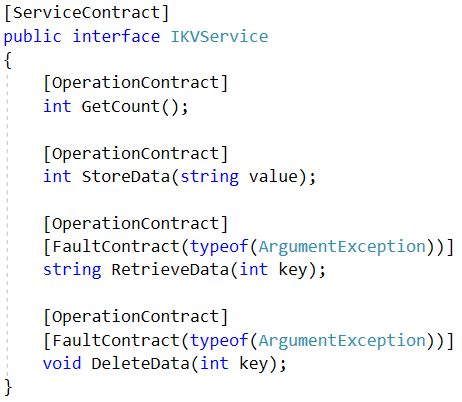
\includegraphics[width=0.7\textwidth]{./figures/ikvservice}
	}
	\caption{Interface IKVService}
	\label{ikvservice}
\end{figure}

O servidor de armazenamento é \textit{stateful} pois tem de guardar os dados de forma persistente. A forma de guardar os dados é em memória.\\
Para a implementação do servidor de armazenamento foi usado o padrão \textit{singleton}. Foi usado este padrão uma vez que é preciso manter estado global.
Os pedidos irão ser atendidos por threads diferentes, pelo que o \textit{ConcurrencyMode} escolhido foi \textit{Multiple}.\\
Assumindo a existência deste serviço na mesma rede com o serviço de \textit{broker}, a comunicação é feita através do protocolo TCP. Foi escolhido este protocolo por ser mais eficiente em relação ao protocolo HTTP e como referido anteriormente, assumindo que ambos os serviços estão na mesma rede. Se mais tarde for requisito estes serviços estarem em redes diferentes, basta mudar o ficheiro de configuração e alterar o \textit{binding} e o \textit{base address} para suportar o protocolo HTTP.

\section{BrokerService} \label{brokerservice}

Para implementar o \textit{broker}, definiu-se a interface IBrokerService, apresentada na figura \ref{ibrokerservice}.

\begin{figure}[h]
	\makebox[\textwidth][c]{
		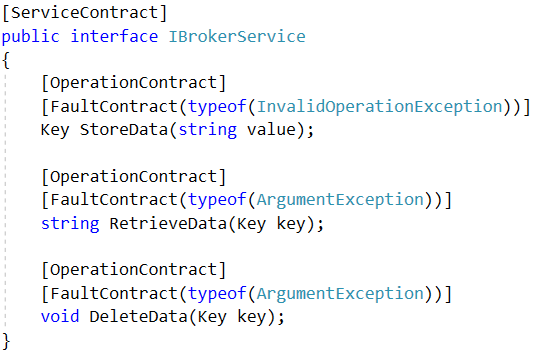
\includegraphics[width=0.7\textwidth]{./figures/ibrokerservice}
	}
	\caption{Interface IBrokerService}
	\label{ibrokerservice}
\end{figure}

Os \textit{brokers} são \textit{stateless} por forma a facilitar o balanceamento de carga. De forma a não ter o objeto em memória foi usado o \textit{InstanceContextMode} \textit{PerCall}.\\
Como o modo é PerCall, ou seja, irá ser criada uma nova instância da classe \textit{BrokerService} a cada chamada, não é necessário garantir controlo de concorrência.\\
Para determinar qual o servidor de armazenamento com maior disponibilidade em termos de volume de dados inseridos, o \textit{broker} pergunta a todos os servidores de armazenamento a carga de cada um. Após ter esta informação, o \textit{broker} ordena os servidores de armazenamento por ordem crescente do volume de dados. Irá escolher os dois primeiros para armazenar o valor nesses servidores. Se algum deles falhar o \textit{broker} tenta guardar no terceiro servidor de armazenamento com menor volume de dados inseridos. Este processo repete-se até conseguir guardar em pelo menos dois servidores de armazenamento. Se conseguir guardar, irá construir um objeto \textit{Key}. Caso contrário irá enviar uma mensagem de exceção a dizer que não foi possível guardar.\\

Para representar a chave de um valor guardado, foi criada a classe \textit{Key} cuja definição se encontra na figura \ref{keydatacontract}

\begin{figure}[h]
	\makebox[\textwidth][c]{
		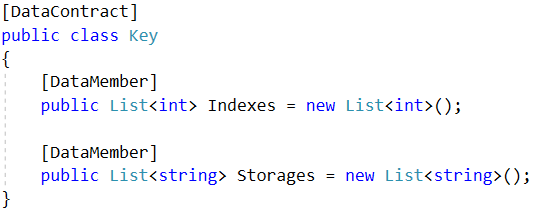
\includegraphics[width=0.7\textwidth]{./figures/key}
	}
	\caption{Classe \textit{Key}}
	\label{keydatacontract}
\end{figure}

Nesta classe é guardada o endereço dos servidores de armazenamento como forma de localização e o índice onde o valor foi guardado dentro do servidor de armazenamento.

Como foi referido na secção \ref{kvservice} é assumido a existência do \textit{broker} na mesma rede que o serviço descrito nessa secção. O \textit{broker} comunica diretamente com o servidor de armazenamento, logo o \textit{binding} usado deve ser o mesmo.
Para que o serviço exposto pelo \textit{broker} seja acessível fora da própria rede, foi usado o protocolo HTTP. O \textit{binding} usado foi o \textit{BasicHttpBinding} porque não é necessário manter sessão ou permitir \textit{callbacks}.

\section{Controlo de Concorrência} \label{concorrencia}

Como o servidor de armazenamento segue o padrão \textit{singleton} irá atender os diferentes pedidos em diferentes \textit{threads}. Como as \textit{threads} irão aceder à mesma instância, é necessário garantir controlo de concorrência. Para garantir o acesso concorrente ao estado dessas instâncias, foi usado a biblioteca \textit{Concurrent} do .NET.\\

\section{Ficheiros de Configuração} \label{configuracao}

De forma a não comprometer o código com os URLs, protocolos, implementações e \textit{bindings}, foi usado ficheiros de configuração.